\documentclass[]{beamer}
\usepackage{tbagrelbeamer}
\usepackage{beamerstylebluesky}
\usepackage{pgfplots}

\begin{document}

\title{Machine learning}
\subtitle{Introduction et utilisation non supervisée}
\author{novembre 2018 @ TELECOM Nancy\\T. \sc{Bagrel}}
\date{}

\begin{frame}
  \titlepage{}
\end{frame}

% \begin{frame}
%   \frametitle{}
%   \framesubtitle{}
% \end{frame}

\begin{frame}
  \frametitle{Définitions}
  \begin{block}{Machine learning}
    Apprentissage automatique / statistique (général)
    \begin{itemize}
      \item supervisé
      \item non supervisé
    \end{itemize}
  \end{block}

  \begin{exampleblock}{Deep learning}
    Réseau de neurones multicouches
  \end{exampleblock}
\end{frame}

\begin{frame}
  \frametitle{Deep learning}
  \framesubtitle{Détail}
  \begin{block}{Plusieurs types de deep learning}
    \begin{itemize}
      \item Deep Neural Network (DNN) : beaucoup de couches de neurones
      \item Convolutional Neural Network (CNN) : découpage du problème en sous-parties, avec un cluster de neurones par sous-partie $\to$ adapté pour le traitement d'images
      \item Deep Belief Network (DBN) : première phase non supervisée puis phase supervisée facilitée par le pré-traitement
    \end{itemize}
  \end{block}

  \alert{Source :}~\url{https://goo.gl/7rcjph}
\end{frame}

\begin{frame}
  \frametitle{Neurone}
  \framesubtitle{Perceptron}
  \begin{center}
    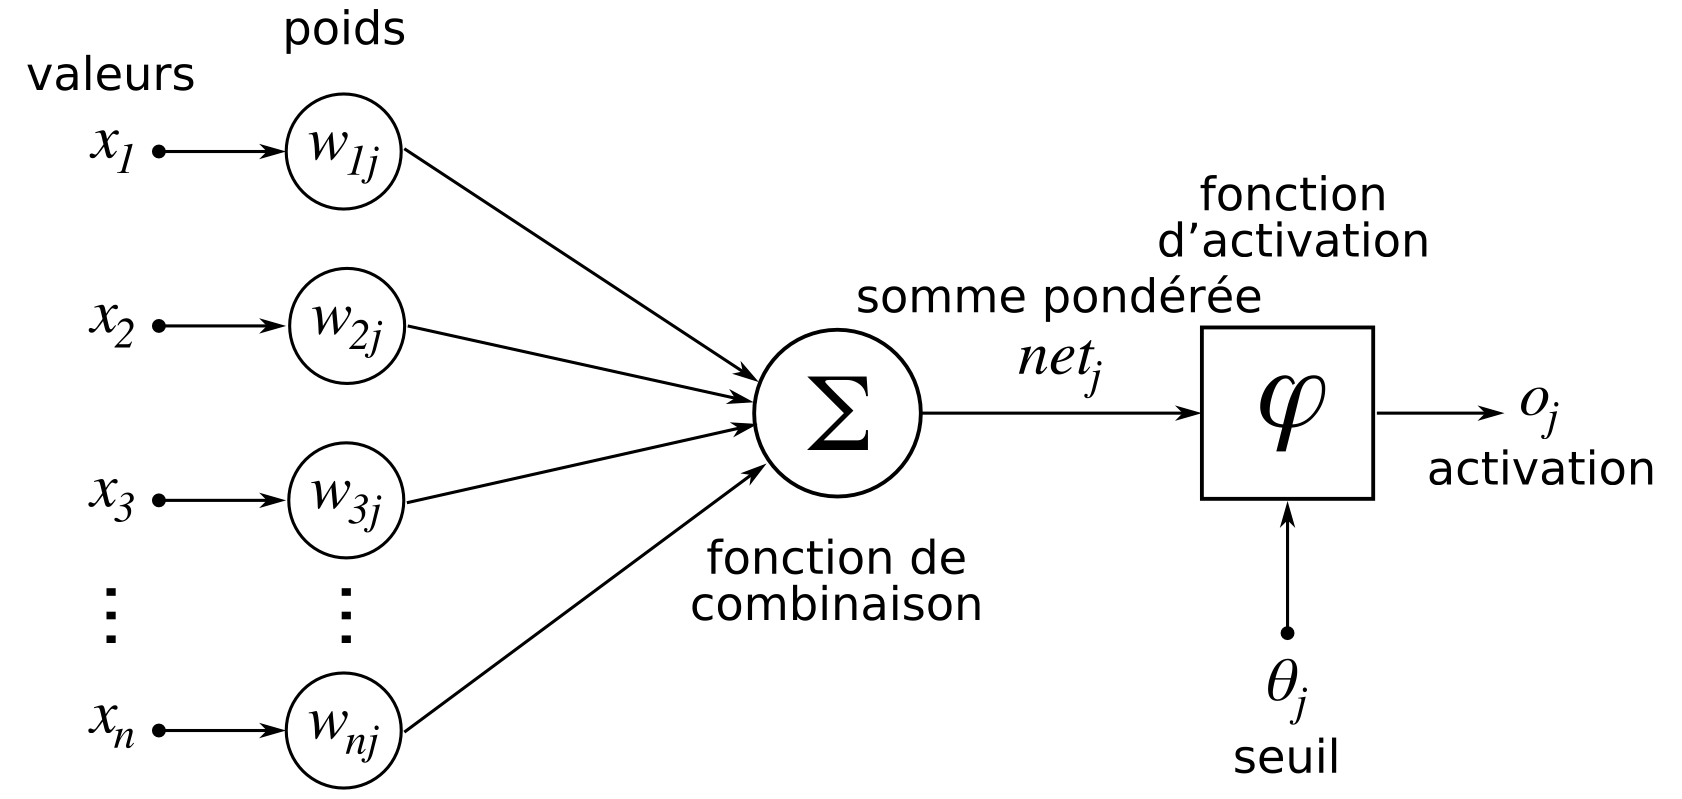
\includegraphics[scale=0.18]{perceptron.png}
  \end{center}
\end{frame}

\begin{frame}
  \frametitle{Machine learning}
  \framesubtitle{Erreur et backpropagation}

  \alert{Important :}~on est ici dans le cadre de l'apprentissage supervisé

  \begin{block}{Erreur}
    \[
      E = f(\text{val}_{\text{attendue}}, \text{val}_{\text{obtenue}})
    \]
  \end{block}

  \begin{block}{Descente du gradient}
    \[
      \Delta w = -\eta \frac{\partial E}{\partial w}
    \]
  \end{block}
\end{frame}

\begin{frame}
  \frametitle{Clustering}
  \framesubtitle{(Machine learning)}

  \begin{block}{Idée}
    Partitionner les données d'entrée sans supervision
  \end{block}

  \begin{alertblock}{Algorithme simple}
    $K$-mean clustering
  \end{alertblock}
\end{frame}

\begin{frame}
  \frametitle{$K$-mean clustering}
  \framesubtitle{Algorithme}
  \begin{exampleblock}{Cas pratique}
    Points sur une surface délimitée en 2D
  \end{exampleblock}

  \begin{block}{Description}
  \begin{enumerate}
    \item On place (aléatoirement) autant de drapeaux (centroids) que l'on veut de groupes (clusters)
    \item Chaque point est rattaché au drapeau le plus proche
    \item On replace le drapeau au centre des points qui lui sont rattachés
    \item Tant que les drapeaux ne sont pas assez stabilisés, on recommence le rattachement (étape \alert{2})
  \end{enumerate}

  \end{block}

\end{frame}

\begin{frame}
  \frametitle{Cas simple}
  \framesubtitle{étape par étape}

  \vfill{}
  \alert{Lancement du programme}
  \vfill{}
\end{frame}

\begin{frame}
  \frametitle{Amélioration}
  \framesubtitle{Laisser l'algorithme trouver le nombre optimal de clusters ?}

  \begin{block}{Contraintes}
    \begin{itemize}
      \item Trouver une définition d'une ``bonne partition''
      \item Fixer des limites à la recherche
    \end{itemize}
  \end{block}
\end{frame}

\begin{frame}
  \frametitle{Définition d'une bonne partition}
  \framesubtitle{(subjectif)}

  \begin{block}{Ma proposition}
       \begin{itemize}
    \item[H] Homogénéité : les groupes doivent avoir des tailles pas trop différentes (pour éviter une partition en $1$ et $10^9$ éléments)
    \item[D] Distinction : les groupes ne doivent pas être trop proches les uns des autres pour pouvoir les distinguer
    \item[S] Stabilité : voir \tt{final\_eps}
    \item[P] Proximité : les éléments d'un cluster doivent être le plus proche possible de leur centroid
  \end{itemize}
  \end{block}
\end{frame}

\begin{frame}
  \frametitle{Comment équilibrer ces facteurs ?}
  %\framesubtitle{}

  \begin{block}{Comportement idéal attendu}
    \begin{itemize}
      \item[H] grand quand les tailles de clusters sont proches
      \item[D] 1 dès que les groupes sont assez éloignés, 0 sinon
      \item[S] ``inverse'' de \tt{final\_eps}
      \item[P] grand quand les points sont proches de leur centroid
    \end{itemize}
  \end{block}
\end{frame}

% \begin{frame}
%   \frametitle{}
%   \framesubtitle{}
% \end{frame}

\begin{frame}
  \frametitle{Implémentation de ces fonctions}
  % \framesubtitle{}
  \vfill{}
  \alert{Code du programme}
  \vfill{}
\end{frame}

\begin{frame}
  \frametitle{Testons !}
  % \framesubtitle{}
  \vfill{}
  \alert{Lancement du programme}
  \vfill{}
\end{frame}

\begin{frame}
  \frametitle{Application à des profils de patients}
  \framesubtitle{Normalisation et distance}

  \begin{block}{Normalisation et centrage}
    Dans le cas où les entrées sont vectorielles, avec des composantes non directement comparables, nécessité d'une normalisation et d'un centrage
  \end{block}

  \begin{alertblock}{Distance}
    La question la plus délicate reste celle de la distance, sans introduire de biais !

    On utilise donc souvent la distance euclidienne, réputée ``neutre''.
  \end{alertblock}

\end{frame}

\begin{frame}
  \frametitle{Réduire la dimension des entrées}
  \framesubtitle{Machine learning -- non supervisé}

  \begin{block}{Principle Composant Analysis}
    Ne capturer que les composantes des vecteurs qui impactent le plus la variance des données
  \end{block}

  \begin{exampleblock}{Singular Value Decomposition}
    Réduire une grande matrice d'entrée en 3 sous-matrices qui contiennent la plus grande partie des informations
  \end{exampleblock}

\end{frame}

\begin{frame}
  \frametitle{Retour sur la backpropagation ?}
  \vfill
  \alert{Si il reste du temps\ldots{}}
  \vfill
\end{frame}

\begin{frame}
  \frametitle{Sources}

  \begin{block}{Remerciements}
    Merci de votre attention !
  \end{block}

  \begin{itemize}
    \item \url{https://goo.gl/W3THM6}
    \item \url{https://goo.gl/Wkbkeo}
    \item \url{https://goo.gl/aJLHRo}
    \item \url{https://goo.gl/QACDyV}
    \item \url{https://goo.gl/aGquwV}
    \item \url{https://goo.gl/24oeED}
    \item \url{https://goo.gl/KLymMw}
    \item \url{https://goo.gl/amYAT2}
  \end{itemize}
\end{frame}

\end{document}
